\documentclass{article}
\usepackage[utf8]{inputenc}
\usepackage{graphicx}
\usepackage[pdftex]{hyperref}

\title{Circuitos digitais}
\author{Amanda Aparcida Machado Goulart - 133569 }
\date{Setembro 2020}

\begin{document}

\maketitle

\section{Laboratório 01}

\subsection{Objetivo}
Implemente um circuito digital que simule um jogo de dados entre dois jogadores.
Como entrada, o circuito possui 3 sinais de entrada para cada jogador que representará um valor entre 1
e 6. Dados os valores das entradas, o jogo deve gerar como saída um de três sinais que indicará a
vitória do jogador 1, a vitória do jogador 2 ou um empate.
Use switches para os sinais de entrada e leds para as saídas.

\subsection{Implementação}

Partindo da sequência lógica para a implementação:

\begin{enumerate}
   \item Entender a lógica do problema
   \item Criar tabela verdade ou mapa de Karnaugh
   \item Gerar expressão correspondente
   \item Desenhar circuito
 \end{enumerate}
\subsubsection{Lógica}
% ######## init table ########
\begin{table}[h]
 \centering
% distancia entre a linha e o texto
 {\renewcommand\arraystretch{1.25}
 \caption{Entrada}
 \begin{tabular}{ l l }
  \cline{1-1}\cline{2-2}  
    \multicolumn{1}{|p{3.850cm}|}{x2,x1,x0 \centering } &
    \multicolumn{1}{p{4.217cm}|}{Valor \centering }
  \\  
  \cline{1-1}\cline{2-2}  
    \multicolumn{1}{|p{3.850cm}|}{001 \centering } &
    \multicolumn{1}{p{4.217cm}|}{1 \centering }
  \\  
  \cline{1-1}\cline{2-2}  
    \multicolumn{1}{|p{3.850cm}|}{010 \centering } &
    \multicolumn{1}{p{4.217cm}|}{2 \centering }
  \\  
  \cline{1-1}\cline{2-2}  
    \multicolumn{1}{|p{3.850cm}|}{011 \centering } &
    \multicolumn{1}{p{4.217cm}|}{3 \centering }
  \\  
  \cline{1-1}\cline{2-2}  
    \multicolumn{1}{|p{3.850cm}|}{100 \centering } &
    \multicolumn{1}{p{4.217cm}|}{4 \centering }
  \\  
  \cline{1-1}\cline{2-2}  
    \multicolumn{1}{|p{3.850cm}|}{101 \centering } &
    \multicolumn{1}{p{4.217cm}|}{5 \centering }
  \\  
  \cline{1-1}\cline{2-2}  
    \multicolumn{1}{|p{3.850cm}|}{110 \centering } &
    \multicolumn{1}{p{4.217cm}|}{6 \centering }
  \\  
  \hline

 \end{tabular} }
\end{table}

\subsubsection{Mapa de Karnaugh}

Primeiramente para fazer a conversão de binário para Grey foi feita o seguinte mapa da karnaugh.

Para y0:

% ######## init table ########
\begin{table}[h]
 \centering
% distancia entre a linha e o texto
 {\renewcommand\arraystretch{1.25}
 \begin{tabular}{ l l l l l }
  \cline{1-1}\cline{2-2}\cline{3-3}\cline{4-4}\cline{5-5}  
    \multicolumn{1}{|p{1.300cm}|}{\begin{center}x2 x1
\end{center}  			


\begin{center}x0
\end{center}} &
    \multicolumn{1}{p{0.700cm}|}{00 \centering } &
    \multicolumn{1}{p{0.700cm}|}{01 \centering } &
    \multicolumn{1}{p{0.700cm}|}{11 \centering } &
    \multicolumn{1}{p{0.650cm}|}{10 \centering }
  \\  
  \cline{1-1}\cline{2-2}\cline{3-3}\cline{4-4}\cline{5-5}  
    \multicolumn{1}{|p{1.300cm}|}{0 \centering } &
    \multicolumn{1}{p{0.700cm}|}{D \centering } &
    \multicolumn{1}{p{0.700cm}|}{1 \centering } &
    \multicolumn{1}{p{0.700cm}|}{1 \centering } &
    \multicolumn{1}{p{0.650cm}|}{0 \centering }
  \\  
  \cline{1-1}\cline{2-2}\cline{3-3}\cline{4-4}\cline{5-5}  
    \multicolumn{1}{|p{1.300cm}|}{1 \centering } &
    \multicolumn{1}{p{0.700cm}|}{1 \centering } &
    \multicolumn{1}{p{0.700cm}|}{0 \centering } &
    \multicolumn{1}{p{0.700cm}|}{D \centering } &
    \multicolumn{1}{p{0.650cm}|}{1 \centering }
  \\  
  \hline

 \end{tabular} }
\end{table}

Resultando em: (x1 !x0)+(!x1 x0)

Para y1:

% ######## init table ########
\begin{table}[h]
 \centering
% distancia entre a linha e o texto
 {\renewcommand\arraystretch{1.25}
 \begin{tabular}{ l l l l l }
  \cline{1-1}\cline{2-2}\cline{3-3}\cline{4-4}\cline{5-5}  
    \multicolumn{1}{|p{1.300cm}|}{\begin{center}x2 x1
\end{center}  			


\begin{center}x0
\end{center}} &
    \multicolumn{1}{p{0.700cm}|}{00 \centering } &
    \multicolumn{1}{p{0.700cm}|}{01 \centering } &
    \multicolumn{1}{p{0.700cm}|}{11 \centering } &
    \multicolumn{1}{p{0.650cm}|}{10 \centering }
  \\  
  \cline{1-1}\cline{2-2}\cline{3-3}\cline{4-4}\cline{5-5}  
    \multicolumn{1}{|p{1.300cm}|}{0 \centering } &
    \multicolumn{1}{p{0.700cm}|}{D \centering } &
    \multicolumn{1}{p{0.700cm}|}{1 \centering } &
    \multicolumn{1}{p{0.700cm}|}{0 \centering } &
    \multicolumn{1}{p{0.650cm}|}{1 \centering }
  \\  
  \cline{1-1}\cline{2-2}\cline{3-3}\cline{4-4}\cline{5-5}  
    \multicolumn{1}{|p{1.300cm}|}{1 \centering } &
    \multicolumn{1}{p{0.700cm}|}{0 \centering } &
    \multicolumn{1}{p{0.700cm}|}{1 \centering } &
    \multicolumn{1}{p{0.700cm}|}{D \centering } &
    \multicolumn{1}{p{0.650cm}|}{1 \centering }
  \\  
  \hline

 \end{tabular} }
\end{table}

Resultando em: (!x2 x1)+(x2 !x1)

Para y2:

% ######## init table ########
\begin{table}[h]
 \centering
% distancia entre a linha e o texto
 {\renewcommand\arraystretch{1.25}
 \begin{tabular}{ l l l l l }
  \cline{1-1}\cline{2-2}\cline{3-3}\cline{4-4}\cline{5-5}  
    \multicolumn{1}{|p{1.300cm}|}{\begin{center}x2 x1
\end{center}  			


\begin{center}x0
\end{center}} &
    \multicolumn{1}{p{0.700cm}|}{00 \centering } &
    \multicolumn{1}{p{0.700cm}|}{01 \centering } &
    \multicolumn{1}{p{0.700cm}|}{11 \centering } &
    \multicolumn{1}{p{0.650cm}|}{10 \centering }
  \\  
  \cline{1-1}\cline{2-2}\cline{3-3}\cline{4-4}\cline{5-5}  
    \multicolumn{1}{|p{1.300cm}|}{0 \centering } &
    \multicolumn{1}{p{0.700cm}|}{D \centering } &
    \multicolumn{1}{p{0.700cm}|}{0 \centering } &
    \multicolumn{1}{p{0.700cm}|}{1 \centering } &
    \multicolumn{1}{p{0.650cm}|}{1 \centering }
  \\  
  \cline{1-1}\cline{2-2}\cline{3-3}\cline{4-4}\cline{5-5}  
    \multicolumn{1}{|p{1.300cm}|}{1 \centering } &
    \multicolumn{1}{p{0.700cm}|}{0 \centering } &
    \multicolumn{1}{p{0.700cm}|}{0 \centering } &
    \multicolumn{1}{p{0.700cm}|}{D \centering } &
    \multicolumn{1}{p{0.650cm}|}{1 \centering }
  \\  
  \hline

 \end{tabular} }
\end{table}

Resultando em: (x2 !x0)+(x2 !x1)

Posteriomente foi feita uma comparação para verificar se são identicos.
\\
\\
\\
\\
\\
\\

% ######## init table ########
\begin{table}[h]
 \centering
% distancia entre a linha e o texto
 {\renewcommand\arraystretch{1.25}
 \begin{tabular}{ l l l l }
  \cline{1-1}\cline{2-2}\cline{3-3}\cline{4-4}  
    \multicolumn{1}{|c|}{00} &
    \multicolumn{1}{c|}{01} &
    \multicolumn{1}{c|}{11} &
    \multicolumn{1}{c|}{10}
  \\  
  \cline{1-1}\cline{2-2}\cline{3-3}\cline{4-4}  
    \multicolumn{1}{|c|}{1} &
    \multicolumn{1}{c|}{0} &
    \multicolumn{1}{c|}{1} &
    \multicolumn{1}{c|}{0}
  \\  
  \hline

 \end{tabular} }
\end{table}

Resultando em (\overline{xi}∙\overline{yi})+(xi∙yi) = xi \oplus yi

Para verificar se é maior ou menor:

Para x2:
% ######## init table ########
\begin{table}[h]
 \centering
% distancia entre a linha e o texto
 {\renewcommand\arraystretch{1.25}
 \begin{tabular}{ l l l l l }
  \cline{1-1}\cline{2-2}\cline{3-3}\cline{4-4}\cline{5-5}  
    \multicolumn{1}{|c|}{x0y0  			

x1y1} &
    \multicolumn{1}{c|}{00} &
    \multicolumn{1}{c|}{01} &
    \multicolumn{1}{c|}{11} &
    \multicolumn{1}{c|}{10}
  \\  
  \cline{1-1}\cline{2-2}\cline{3-3}\cline{4-4}\cline{5-5}  
    \multicolumn{1}{|c|}{00} &
    \multicolumn{1}{c|}{0} &
    \multicolumn{1}{c|}{1} &
    \multicolumn{1}{c|}{0} &
    \multicolumn{1}{c|}{0}
  \\  
  \cline{1-1}\cline{2-2}\cline{3-3}\cline{4-4}\cline{5-5}  
    \multicolumn{1}{|c|}{01} &
    \multicolumn{1}{c|}{1} &
    \multicolumn{1}{c|}{1} &
    \multicolumn{1}{c|}{1} &
    \multicolumn{1}{c|}{1}
  \\  
  \cline{1-1}\cline{2-2}\cline{3-3}\cline{4-4}\cline{5-5}  
    \multicolumn{1}{|c|}{11} &
    \multicolumn{1}{c|}{0} &
    \multicolumn{1}{c|}{1} &
    \multicolumn{1}{c|}{0} &
    \multicolumn{1}{c|}{0}
  \\  
  \cline{1-1}\cline{2-2}\cline{3-3}\cline{4-4}\cline{5-5}  
    \multicolumn{1}{|c|}{10} &
    \multicolumn{1}{c|}{0} &
    \multicolumn{1}{c|}{0} &
    \multicolumn{1}{c|}{0} &
    \multicolumn{1}{c|}{0}
  \\  
  \hline

 \end{tabular} }
\end{table}

Para y2:

% ######## init table ########
\begin{table}[h]
 \centering
% distancia entre a linha e o texto
 {\renewcommand\arraystretch{1.25}
 \begin{tabular}{ l l l l l }
  \cline{1-1}\cline{2-2}\cline{3-3}\cline{4-4}\cline{5-5}  
    \multicolumn{1}{|c|}{x0y0  			

x1y1} &
    \multicolumn{1}{c|}{00} &
    \multicolumn{1}{c|}{01} &
    \multicolumn{1}{c|}{11} &
    \multicolumn{1}{c|}{10}
  \\  
  \cline{1-1}\cline{2-2}\cline{3-3}\cline{4-4}\cline{5-5}  
    \multicolumn{1}{|c|}{00} &
    \multicolumn{1}{c|}{1} &
    \multicolumn{1}{c|}{1} &
    \multicolumn{1}{c|}{1} &
    \multicolumn{1}{c|}{1}
  \\  
  \cline{1-1}\cline{2-2}\cline{3-3}\cline{4-4}\cline{5-5}  
    \multicolumn{1}{|c|}{01} &
    \multicolumn{1}{c|}{1} &
    \multicolumn{1}{c|}{1} &
    \multicolumn{1}{c|}{1} &
    \multicolumn{1}{c|}{1}
  \\  
  \cline{1-1}\cline{2-2}\cline{3-3}\cline{4-4}\cline{5-5}  
    \multicolumn{1}{|c|}{11} &
    \multicolumn{1}{c|}{1} &
    \multicolumn{1}{c|}{1} &
    \multicolumn{1}{c|}{1} &
    \multicolumn{1}{c|}{1}
  \\  
  \cline{1-1}\cline{2-2}\cline{3-3}\cline{4-4}\cline{5-5}  
    \multicolumn{1}{|c|}{10} &
    \multicolumn{1}{c|}{1} &
    \multicolumn{1}{c|}{1} &
    \multicolumn{1}{c|}{1} &
    \multicolumn{1}{c|}{1}
  \\  
  \hline

 \end{tabular} }
\end{table}

Para y1:
\begin{figure}[!h]
\centering
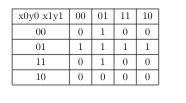
\includegraphics[width=6cm]{y1.jpeg}
\label{fig:CL_logo}
\end{figure}


Para x1:

\begin{figure}[!h]
\centering
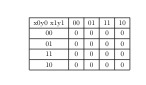
\includegraphics[width=6cm]{x1.jpeg}
\label{fig:CL_logo}
\end{figure}
Resultando em: (\overline{x2}∙y2)+(\overline{x2}∙\overline{x1}∙y1)+(\overline{x2}∙\overline{x1}∙\overline{x0}∙y0)+(x2∙y1∙\overline{x0}∙y0)+(y2∙\overline{x1}∙y1)+(y2∙\overline{x1}∙\overline{x0}∙y0)+(y2∙y1∙\overline{x0}∙y0)
\subsection{Circuito}

\begin{figure}[!h]
\centering
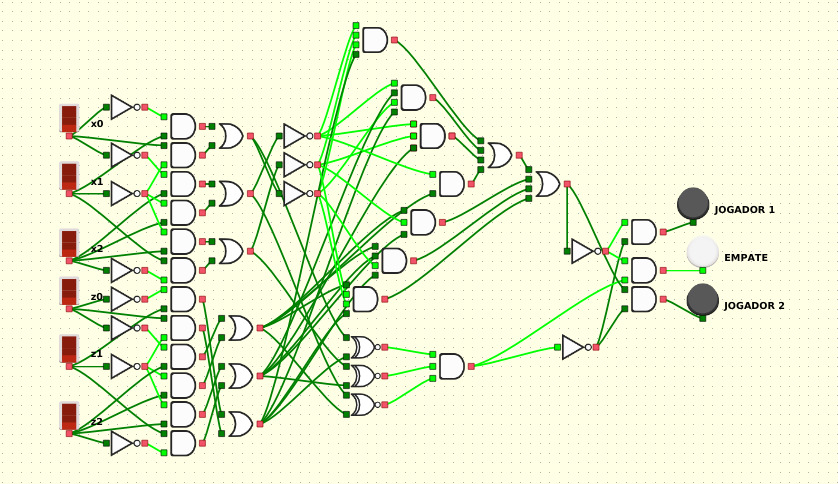
\includegraphics[width=15cm]{circuito.jpeg}
\caption{Circuito do laboratório 01}
\label{fig:CL_logo}
\end{figure}

O arquivo .panda pode ser encontrado no seguinte \href{https://github.com/aamgoulart/circuitosDigitais}{repositório}

\end{document}